\chapter{Selective sweeps on different pigmentation genes mediate convergent evolution of island melanism in two incipient bird species}

\textit{Content of this chapter was published in PLoS Genetics (2022) under the title ``Selective sweeps on different pigmentation genes mediate convergent evolution of island melanism in two incipient bird species" by Leonardo Campagna, Ziyi Mo, Adam Siepel and J. Albert C. Uy. L.C. conceptualized the study, curated data, performed formal analyses, developed methodology and wrote the manuscript. Z.M. characterized selective sweeps in the bird populations using the SIA method, developed methodology and edited the manuscript. A.S. developed methodology and edited the manuscript. J.A.C.U. conceptualized the study, curated data, performed formal analyses, developed methodology and wrote the manuscript.}

\section{Abstract}

Insular organisms often evolve predictable phenotypes, like flightlessness, extreme body sizes, or increased melanin deposition. The evolutionary forces and molecular targets mediating these patterns remain mostly unknown. Here we study the Chestnut-bellied Monarch (\textit{Monarcha castaneiventris}) from the Solomon Islands, a complex of closely related subspecies in the early stages of speciation. On the large island of Makira \textit{M. c. megarhynchus} has a chestnut belly, whereas on the small satellite islands of Ugi, and \ac{SA/SC} \textit{M. c. ugiensis} is entirely iridescent blue-black (i.e., melanic). Melanism has likely evolved twice, as the Ugi and \ac{SA/SC} populations were established independently. To investigate the genetic basis of melanism on each island we generated whole genome sequence data from all three populations. Non-synonymous mutations at the \textit{MC1R} pigmentation gene are associated with melanism on \ac{SA/SC}, while \textit{ASIP}, an antagonistic ligand of \textit{MC1R}, is associated with melanism on Ugi. Both genes show evidence of selective sweeps in traditional summary statistics and statistics derived from the \acf{ARG}. Using the \ac{ARG} in combination with machine learning, we inferred selection strength, timing of onset and allele frequency trajectories. \textit{MC1R} shows evidence of a recent, strong, soft selective sweep. The region including \textit{ASIP} shows more complex signatures; however, we find evidence for sweeps in mutations near \textit{ASIP}, which are comparatively older than those on \textit{MC1R} and have been under relatively strong selection. Overall, our study shows convergent melanism results from selective sweeps at independent molecular targets, evolving in taxa where coloration likely mediates reproductive isolation with the neighboring chestnut-bellied subspecies.

\section{Introduction}

% \begin{figure}
%     \centering
%     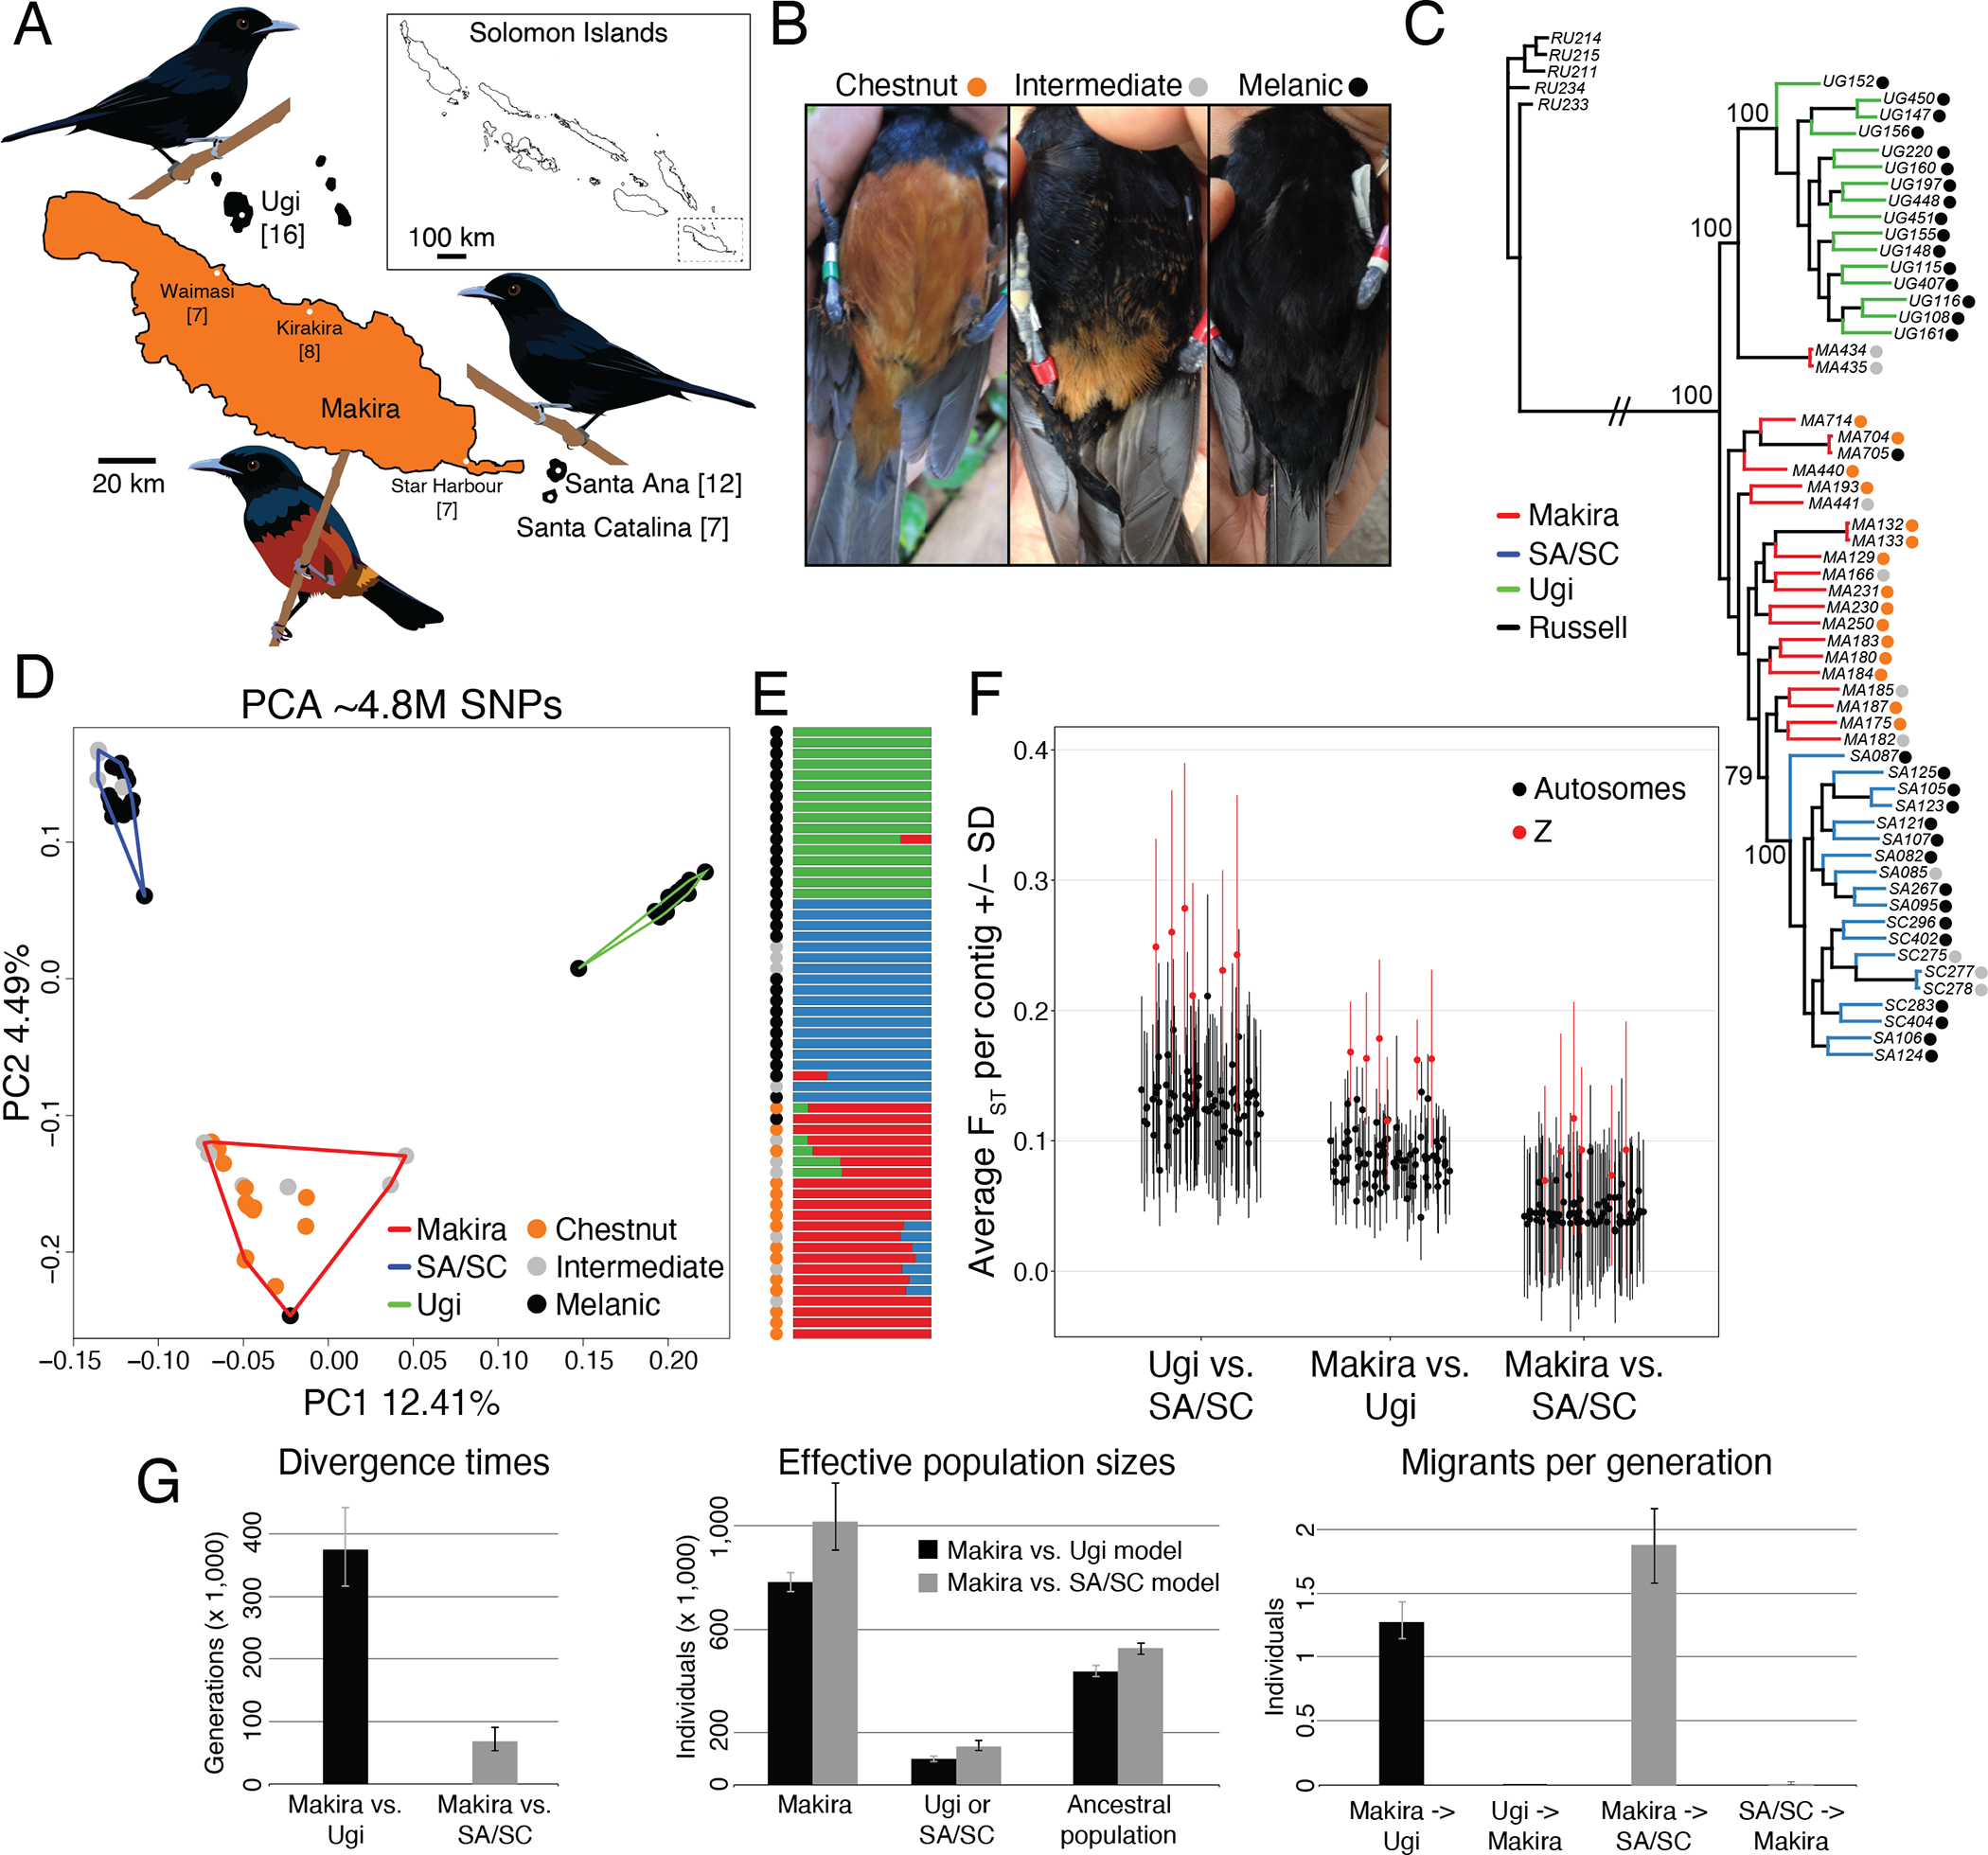
\includegraphics[width=\textwidth]{monarcha_figs/mon_F1.PNG}
%     \caption{Caption}
%     \label{fig:mon-F1}
% \end{figure}

\section{Results}

\section{Discussion}

\section{Materials and methods}

\section{Supplementary material}
Supporting information is available at \href{https://journals.plos.org/PLOSGENETICS/article?id=10.1371/journal.pgen.1010474#sec017}{\textit{PLoS Genetics} online}. The computer code for this project has been deposited in GitHub repos, \href{https://github.com/CshlSiepelLab/bird_capuchino_analysis}{\texttt{bird\_capuchino\_analysis}} and \href{https://github.com/CshlSiepelLab/arg-selection}{\texttt{arg-selection}}. Genomic data have been archived in GenBank (BioProject ID PRJNA835722).